\documentclass[a4paper,12pt]{book}
\usepackage[polish]{babel}	%konieczny do polskich znak�w
\usepackage[latin2]{inputenc}   % lub utf8
\usepackage[T1]{fontenc}
\usepackage{graphicx}
\usepackage{anysize}
\usepackage{enumerate}
\usepackage{times}
\usepackage{tipa}
\usepackage{tipx}
\usepackage{extsizes}
\usepackage{tikz}
\usetikzlibrary{arrows,decorations.markings}

%\marginsize{left}{right}{top}{bottom}
\marginsize{3cm}{3cm}{3.2cm}{2.5cm}
%\sloppy

\begin{document}
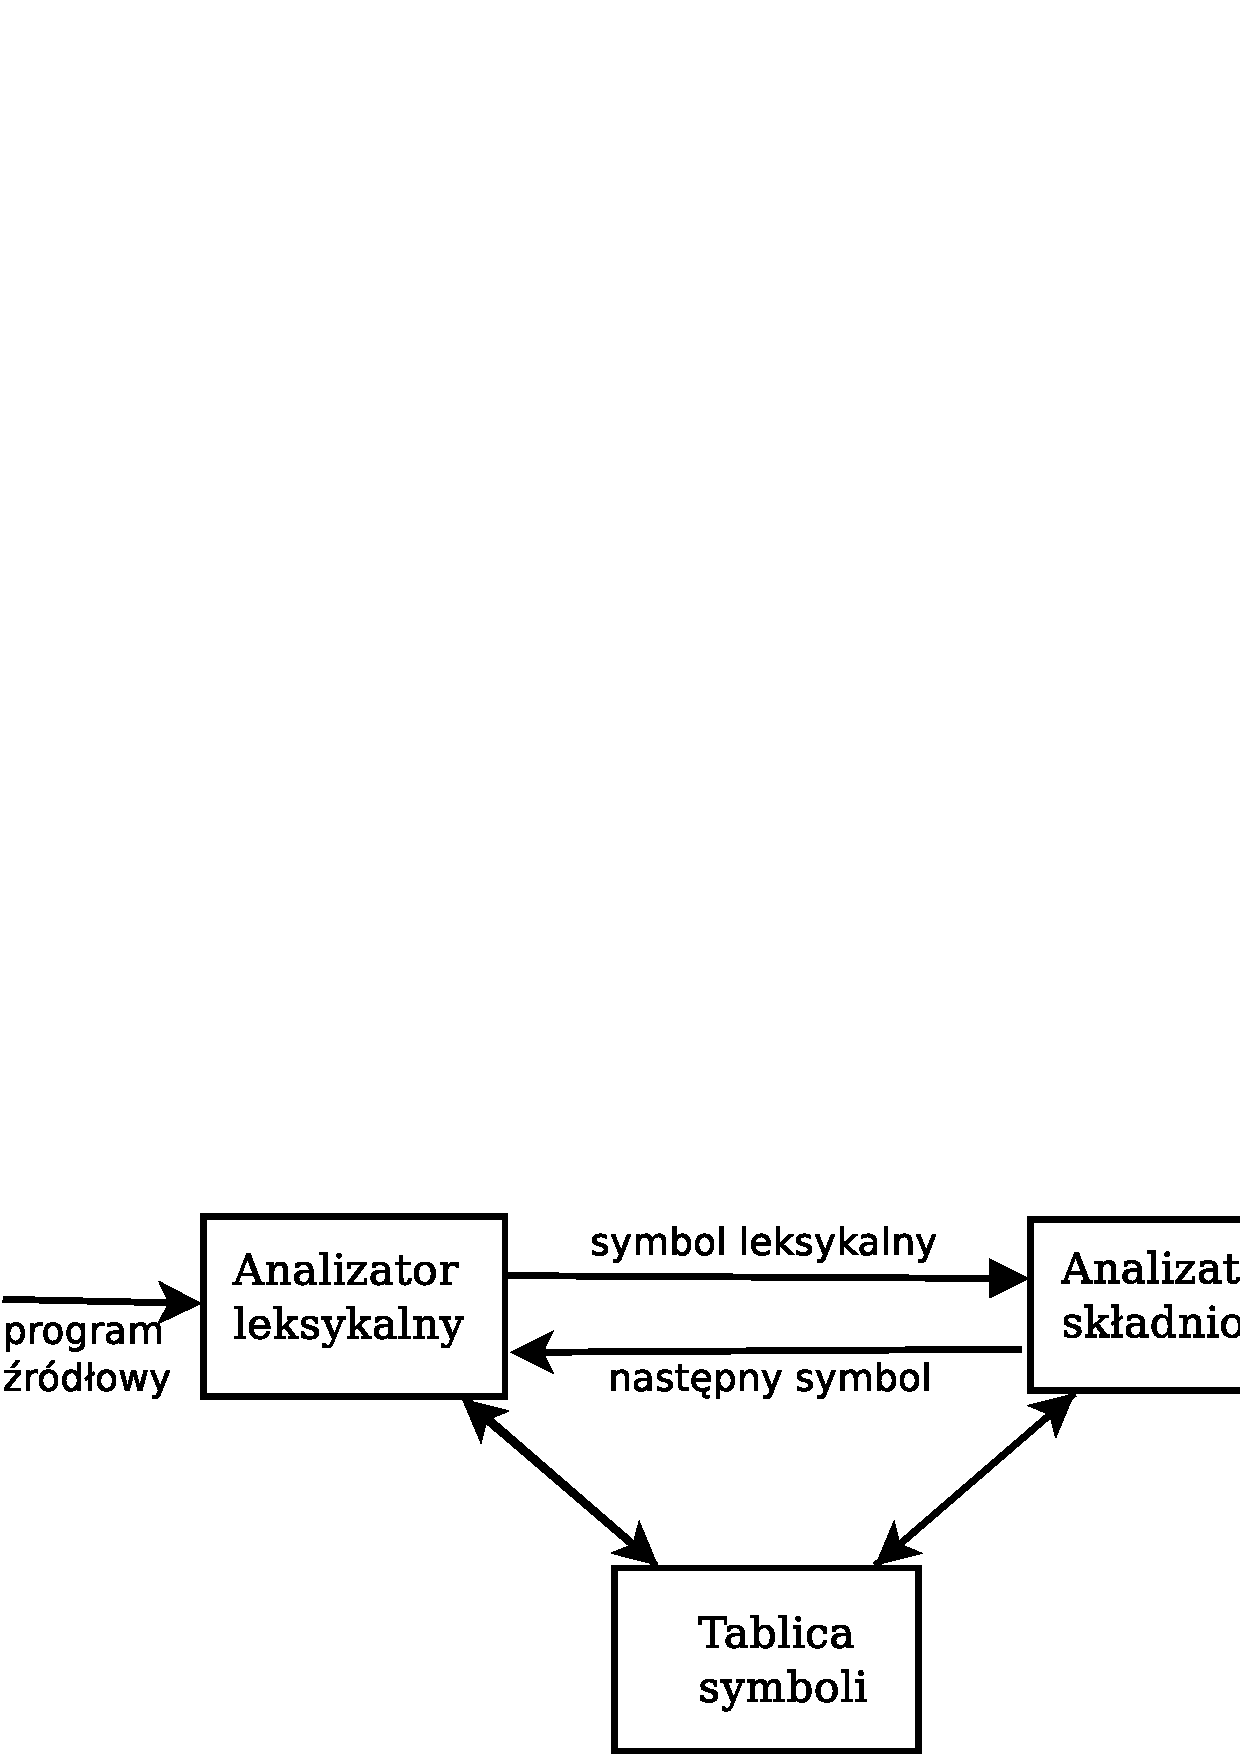
\includegraphics[width=\textwidth]{Diagram1.pdf}
\\
\\\\\\\\\\

\begin{figure}[!htb]
\centering
\begin{tikzpicture}
\node at (0,0) {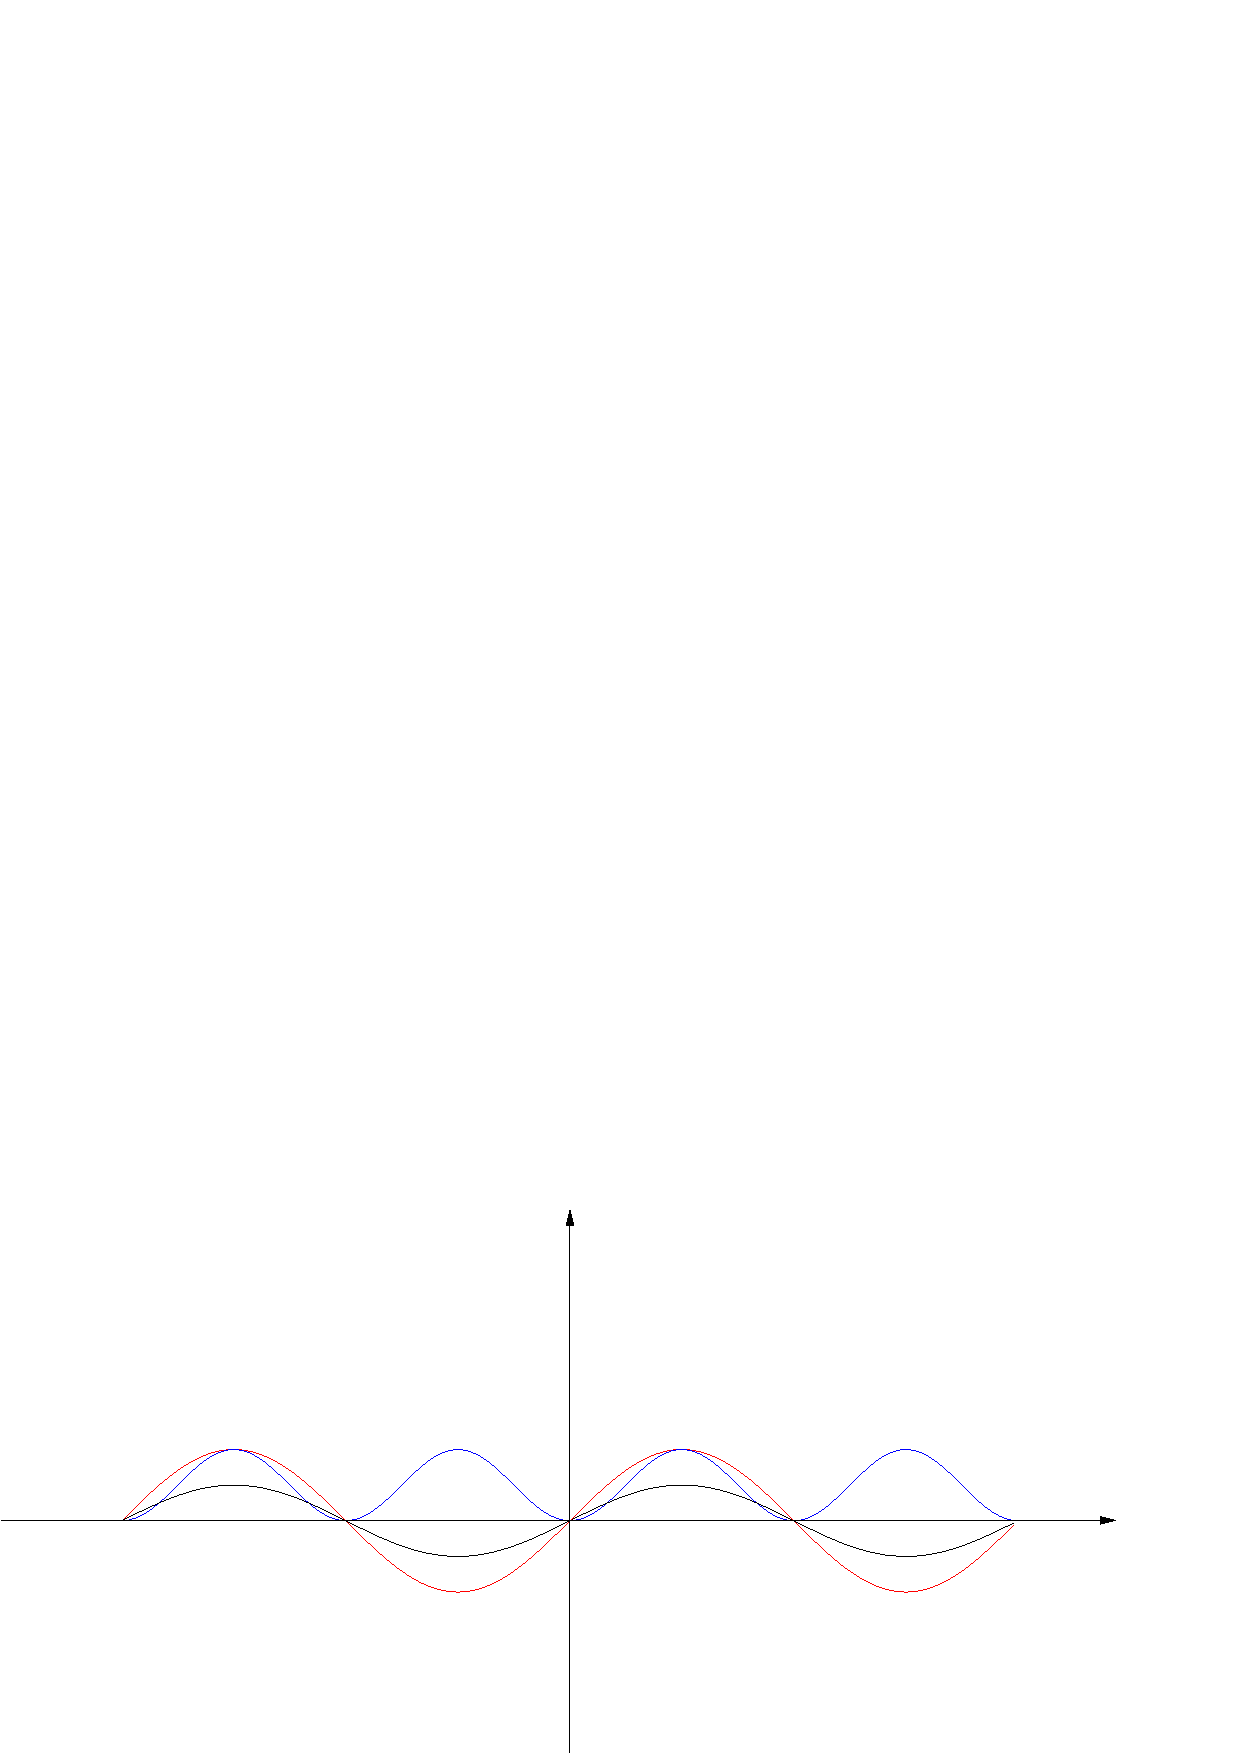
\includegraphics[width=\textwidth]{f1.pdf}};
\node at (4.8,-2.0) {$f(x) = \sin(x)$};
\node at (4.8,0.8) {$g(x) = \sin^2(x)$};
\node at (1.9,-0.9) {$h(x) = \frac{sin(x)}{2}$};
\end{tikzpicture}
\caption{Wykresy funkcji}
\label{fig:funkcje}
\end{figure}



\begin{figure}[!htb]
\centering
\begin{tikzpicture}
\node at (0,0) {\includegraphics[width=\textwidth]{fig4_4.pdf}};
\node at (4.3,-0.8) {$f(x) = \sin(x)$};
\node at (4.3,1.6) {$g(x) = \sin^2(x)$};
\node at (1.4,-0.1) {$h(x) = \frac{sin(x)}{2}$};
\draw[->,>=stealth] (-6,0.33)--(6,0.33) node[right]{$x$};
\draw[->,>=stealth] (0.085,-3)--(0.085,3) node[above]{$y$};
\end{tikzpicture}
\caption{Wykresy funkcji}
\label{fig:funkcje}
\end{figure}

\begin{figure}
\includegraphics[width=\textwidth]{f2.pdf}
\end{figure}

\end{document}